\documentclass[11pt]{article}

\usepackage[lmargin=0.75in, rmargin=1in, tmargin=1.25in, bmargin=1in]{geometry}
\usepackage[english]{babel}
\usepackage[utf8]{inputenc}

\usepackage{amsfonts}
\usepackage{amsmath}
\usepackage{bm}
\usepackage{booktabs}
\usepackage[labelsep=period]{caption}
\usepackage{enumitem}
\usepackage{fancyhdr}
\usepackage{graphicx}
\usepackage{lastpage}
\usepackage{listings}
\usepackage[svgnames]{xcolor}
\usepackage{float}
\usepackage{array}
\usepackage{subcaption}
\newcolumntype{P}[1]{>{\centering\arraybackslash}p{#1}}
\newcolumntype{M}[1]{>{\centering\arraybackslash}m{#1}}

% For formatting C++ code listings ---------------------------
\lstdefinestyle{customCpp}{
    language=C++,
    keywordstyle=\color{RoyalBlue},
    basicstyle=\footnotesize\ttfamily,
    commentstyle=\color{Green}\ttfamily,
    rulecolor=\color{black},
    numbers=left,
    numberstyle=\tiny\color{gray},
    stepnumber=1,
    numbersep=8pt,
    showstringspaces=false,
    breaklines=true,
    frame = tb,
    belowcaptionskip=5pt,
    belowskip=3em,
    gobble=10,
}

% For turning enumerated lists into Problem titles --------------
\renewcommand{\labelenumi}{\textbf{\arabic{enumi}.}}
\renewcommand{\labelenumii}{(\alph{enumii})}
\setlength\parindent{24pt}
\newcommand{\forceindent}{\leavevmode{\parindent=1em\indent}}

% Enumerated list indents:
% Problems:    [leftmargin=0.9in]
% Subproblems: [leftmargin=0.3in]


% Document Details ----------------------------------------------
\author{Eli Case}
\title{MECH 450 -- Project 1}
\date{September, 1, 2023}
\makeatletter


% Setup headers -------------------------------------------------
\pagestyle{fancy}
\fancyhf{} % Clear the headers and footers
\lhead{\@author}
\chead{\@title}
\rhead{\@date}
\cfoot{Page \thepage\ of \pageref{LastPage}}
\setlength{\headheight}{15pt}
\setlength{\headsep}{20pt}

\fancypagestyle{plain}{
	\fancyhf{}
	\setlength{\headheight}{15pt}
	\setlength{\headsep}{0pt}
	\renewcommand{\headrulewidth}{0pt}
	\cfoot{\vspace{2mm}Page \thepage\ of \pageref{LastPage}}
}


\begin{document}
\flushleft
\thispagestyle{plain}

From: \@author

Date: \@date

Subject: \@title

\makeatother
\medskip
\hrule
\medskip

\begin{enumerate}[leftmargin=0.3in]

   \item % Problem 1

   \begin{enumerate}[leftmargin=0.3in]
      \forceindent To install \text{{\fontfamily{cmtt}\selectfont OMPL}} and \text{{\fontfamily{cmtt}\selectfont OMPL.app}}, I setup the \text{{\fontfamily{cmtt}\selectfont docker}} environment. Once I was able to configure my machine correctly for \text{{\fontfamily{cmtt}\selectfont docker}}, the installation process was straight-foward and took about 20 minutes.
   \end{enumerate} % End of Problem 1 subpoints

   \item % Problem 2   
   \begin{enumerate}[leftmargin=0.3in]
   
    \forceindent Based on these timings, we can compare the demos for car-like systems. The \text{\fontfamily{cmtt}\selectfont DynamicCarPlanning} demo appears to have been the most difficult demo overall, since it required about 5 times longer to find a solution than the nearest algorithm, \text{\fontfamily{cmtt}\selectfont RigidBodyPlanningWithControls}. Additionally, \text{\fontfamily{cmtt}\selectfont DynamicCarPlanning} required about 10 more states than the nearest algorithm,  \text{\fontfamily{cmtt}\selectfont RigidBodyPlanningWithControls}. Notably, both the car-like planning algorithms with controls and no obstacles took much longer time and more states to find a solution than the car-like planning algorithm without controls and no obstacles, suggesting that adding controls to a system drastically increases the motion planning complexity.

    \forceindent The \text{\fontfamily{cmtt}\selectfont RigidBodyPlanning} demo took the least amount of time, along with \text{\fontfamily{cmtt}\selectfont GeometricCarPlanning} having the second shortest time. These algorithms also required the least amount of created states. This finding is intuitive, as these planning demos occurred in spaces without obstacles.

    \forceindent From comparing the demos for rigid-body planning, \text{\fontfamily{cmtt}\selectfont SE2RigidBodyPlanning} had the longest time out of the rigid body demos and required the most states. This result is expected, since this demo occurred in 3D space with obstacles, as compared to 2D space with obstacles and 3D space without obstacles for the other rigid body demos. 

    \forceindent Overall, the most difficult problem out of the demos seems to be planning for systems with controls. Furthermore, planning in 3D space is more expensive than planning in a 2D space with a comparable environment, as expected.

       \begin{table}[H]
       \centering
       \begin{tabular}{|M{7cm}|M{5cm}|M{4cm}|}
           \hline
           \multicolumn{3}{|c|}{Performance Evaluation of the Six Demo Programs} \\
           \hline
           Demo Program & Average Time to Find Solution [s] & Number of Created States\\
           \hline
           \text{\fontfamily{cmtt}\selectfont RigidBodyPlanning} & 0.001105 & 102\\
           \hline
           \text{{\fontfamily{cmtt}\selectfont SE2RigidBodyPlanning}} & 0.17146 & 879\\
           \hline
           \text{{\fontfamily{cmtt}\selectfont SE3RigidBodyPlanning}} & 1.391743 & 29095\\
           \hline
           \text{{\fontfamily{cmtt}\selectfont GeometricCarPlanning --easyplan}} & 0.019515 & 4373\\
           \hline
           \text{{\fontfamily{cmtt}\selectfont RigidBodyPlanningWithControls}} & 2.23453 & 173456\\
           \hline
           \text{{\fontfamily{cmtt}\selectfont DynamicCarPlanning}} & 40.084117 & 1303070\\
           \hline
       \end{tabular}
       \caption{Demo Program Performance}
       \label{tab:1}
       \end{table}

   \end{enumerate}    
   
   \item % Problem 3   
   \begin{enumerate}[leftmargin=0.3in]

   \forceindent Below in Table \ref{tab:2}, the solution time and created states are summarized for each problem configuration. Note that each problem used the \text{\fontfamily{cmtt}\selectfont KPIECE1} planner to easily compare results. Based on the number of states formed and the time to find a solution,  \text{\fontfamily{cmtt}\selectfont 3D/TwistyCool} appears to be the most difficult problem. It should be noted that  \text{\fontfamily{cmtt}\selectfont 3D/TwistyCool} failed using the \text{\fontfamily{cmtt}\selectfont KPIECE1} planner.
   
   \forceindent Next, the problem configuration \text{\fontfamily{cmtt}\selectfont 3D/Home} had the largest number of created states. This result is intuitive, as the object being moved has a complex shape in an environment with low clearance between obstacles. The time to compute the solution for \text{\fontfamily{cmtt}\selectfont 3D/Home} was shorter than for \text{\fontfamily{cmtt}\selectfont 3D/Abstract}, despite the fact that \text{\fontfamily{cmtt}\selectfont 3D/Abstract} required less states to solve. This result is attributed to the fact that \text{\fontfamily{cmtt}\selectfont Abstract} has a complex environment than  \text{\fontfamily{cmtt}\selectfont Home} with more complex obstacles, but a less complex object to move. Lastly, the 2D problem configurations required less states and time to solve, which is intuitive since there is less free space to plan in when there are less spatial dimensions.

       \begin{table}[H]
       \centering
       \begin{tabular}{|M{5cm}|M{5cm}|M{4cm}|M{2cm}|}
           \hline
           \multicolumn{4}{|c|}{Performance Evaluation of the Five Problem Configurations} \\
           \hline
           Problem Configuration & Time to Find Solution [s] & Number of Created States & Planner\\
           \hline
           \text{\fontfamily{cmtt}\selectfont 2D/BugTrap\text\_planar.cfg} & 0.017708 & 453  & \text{{\fontfamily{cmtt}\selectfont KPIECE1}} \\
           \hline
           \text{{\fontfamily{cmtt}\selectfont 2D/UniqueSolutionMaze.cfg}} & 0.714159 & 2497 & \text{\fontfamily{cmtt}\selectfont KPIECE1}\\
           \hline
           \text{{\fontfamily{cmtt}\selectfont 3D/Abstract.cfg}} & 7.532828 & 26579 & \text{\fontfamily{cmtt}\selectfont KPIECE1}\\
           \hline
           \text{{\fontfamily{cmtt}\selectfont 3D/TwistyCool.cfg}} & 10.090663 & 70240 & \text{\fontfamily{cmtt}\selectfont KPIECE1}\\
           \hline
           \text{{\fontfamily{cmtt}\selectfont 3D/Home.cfg}} & 4.921847 & 42322 & \text{\fontfamily{cmtt}\selectfont KPIECE1}\\
           \hline
       \end{tabular}
       \caption{Demo Program Timings}
       \label{tab:2}
       \end{table}

   \end{enumerate}    
   
   \item % Problem 4   
   \begin{enumerate}[leftmargin=0.3in]
\forceindent To evaluate planner performance, the success of the planner across the 5 problem configurations is considered. The \text{\fontfamily{cmtt}\selectfont PRM} planner was not able to exactly solve \text{\fontfamily{cmtt}\selectfont 3D/TwistyCool.cfg} or \text{\fontfamily{cmtt}\selectfont 3D/Abstract.cfg}. \text{\fontfamily{cmtt}\selectfont RRT-Connect} also failed on these problems.  \text{\fontfamily{cmtt}\selectfont KPIECE1} and  \text{\fontfamily{cmtt}\selectfont RRT} were able to solve 4 of the 5 problem configurations, being the most verstile. Generally, the planners with ranom sampling could have better performance if the sampling happened to be better, while  \text{\fontfamily{cmtt}\selectfont KPIECE1} had more consistent but sometimes worse performance. 
   \end{enumerate}    
   
   \item % Problem 5 
   \begin{enumerate}[leftmargin=0.3in]
\forceindent From increasing the goal bias, it appears a higher goal bias places more weight on achieving a path that is close to the straight goal distance. Too much goal bias seems to degrade the obstacle navigation performance. Increasing the range parameter seems to be analogous to increasing the sensor range. In the \text{\fontfamily{cmtt}\selectfont 3D/TwistyCool.cfg} problem for example, increasing the range allows some planners to be able to find a solution, which is intuitive, since increasing the range allows the object to more easily see the other room between the wall gap. Lastly, increasing the max number of neighbors decreases the number of sampling states, as each state can be connected to more states, reducing the need to sample a large number of states. 
   \end{enumerate}    
   
   \item % Problem 6
   \begin{enumerate}[leftmargin=0.3in]
\forceindent First, the success rate for the various planners on each problem need to be discussed. Figure \ref{fig:1} gives the cdf statistics for each problem configuration. \text{\fontfamily{cmtt}\selectfont Home} and \text{\fontfamily{cmtt}\selectfont Abstract} did not achieve a success rate over 90 \% for some of the planners, despite increasing the time limit to 10 minutes for all problem configurations. As a result, the issue with the planners solving these problem configurations is assumed to be an issue with my computer architecture. Likely, a limitation imposed by the processor or memory making the benchmarking difficult to complete within a reasonable time constraint. 

       \begin{figure}[H]
          \centering
          \begin{subfigure}[b]{0.3\textwidth}
             \centering
             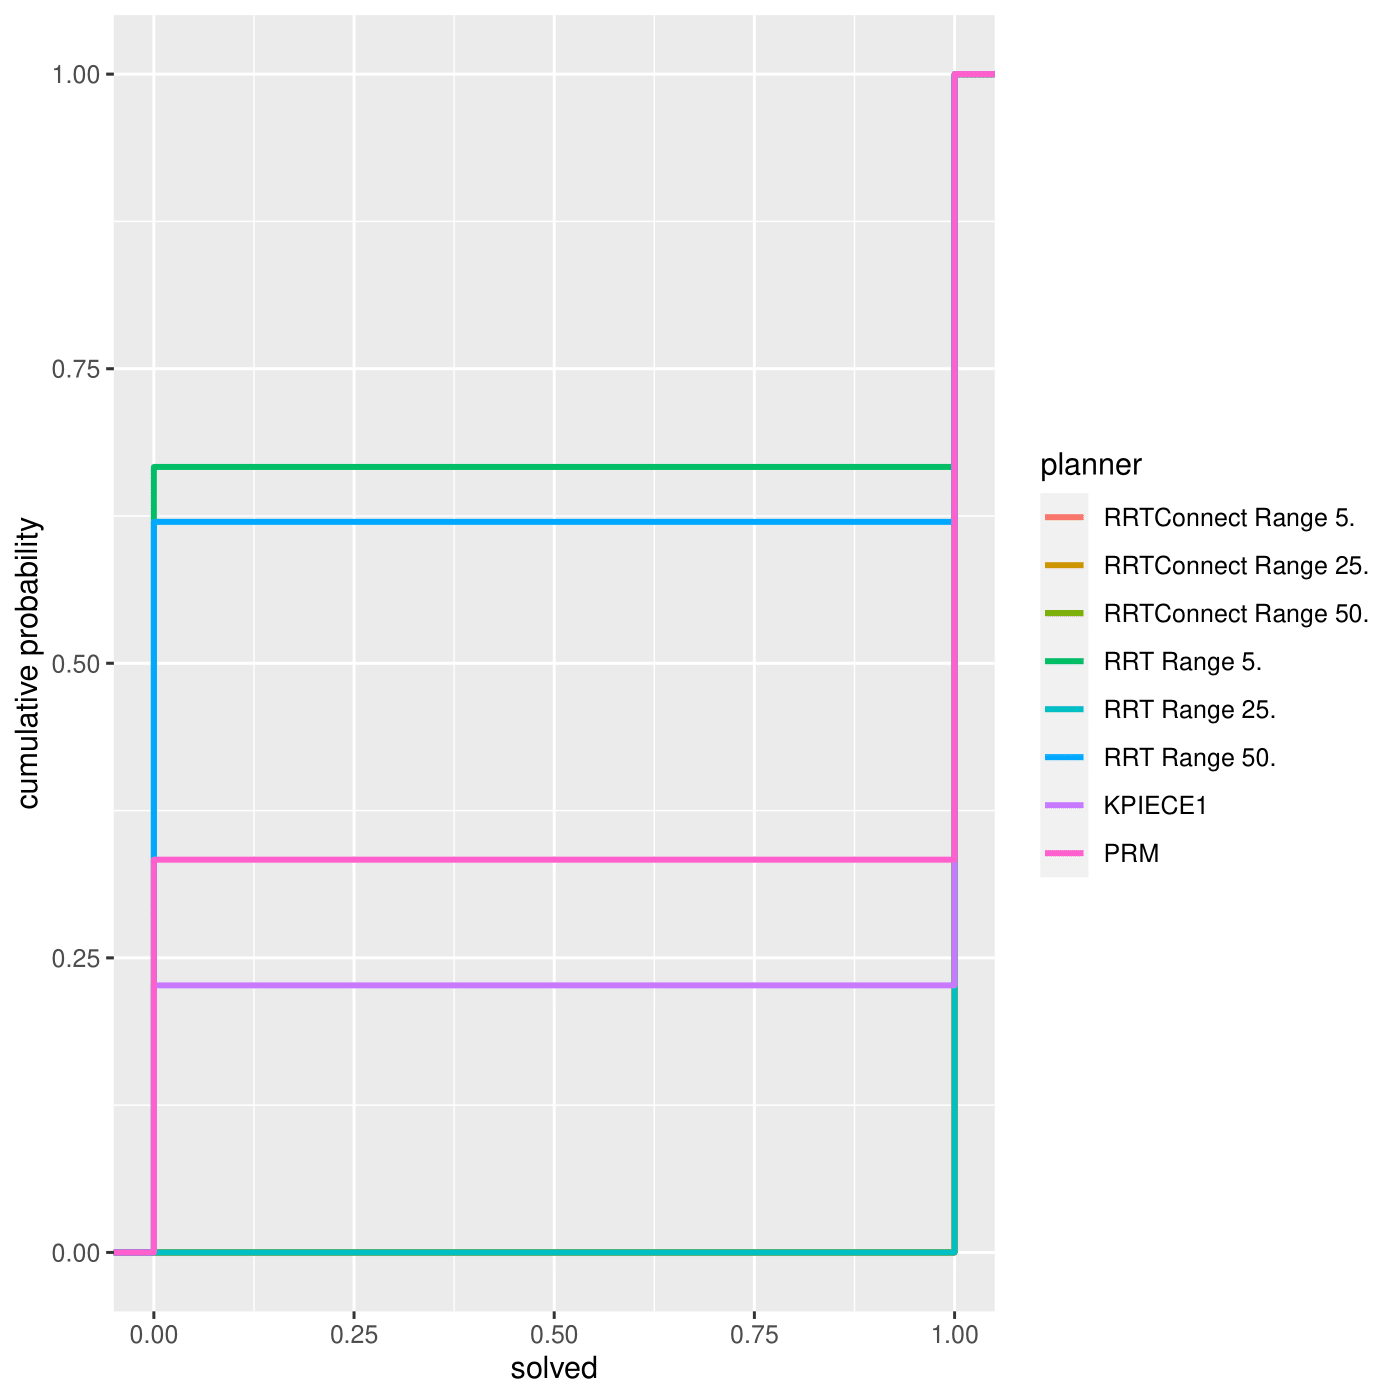
\includegraphics[width=\textwidth]{figures/home_solved-1.png}
             \caption{Home}
           \end{subfigure}
           \begin{subfigure}[b]{0.3\textwidth}
              \centering
              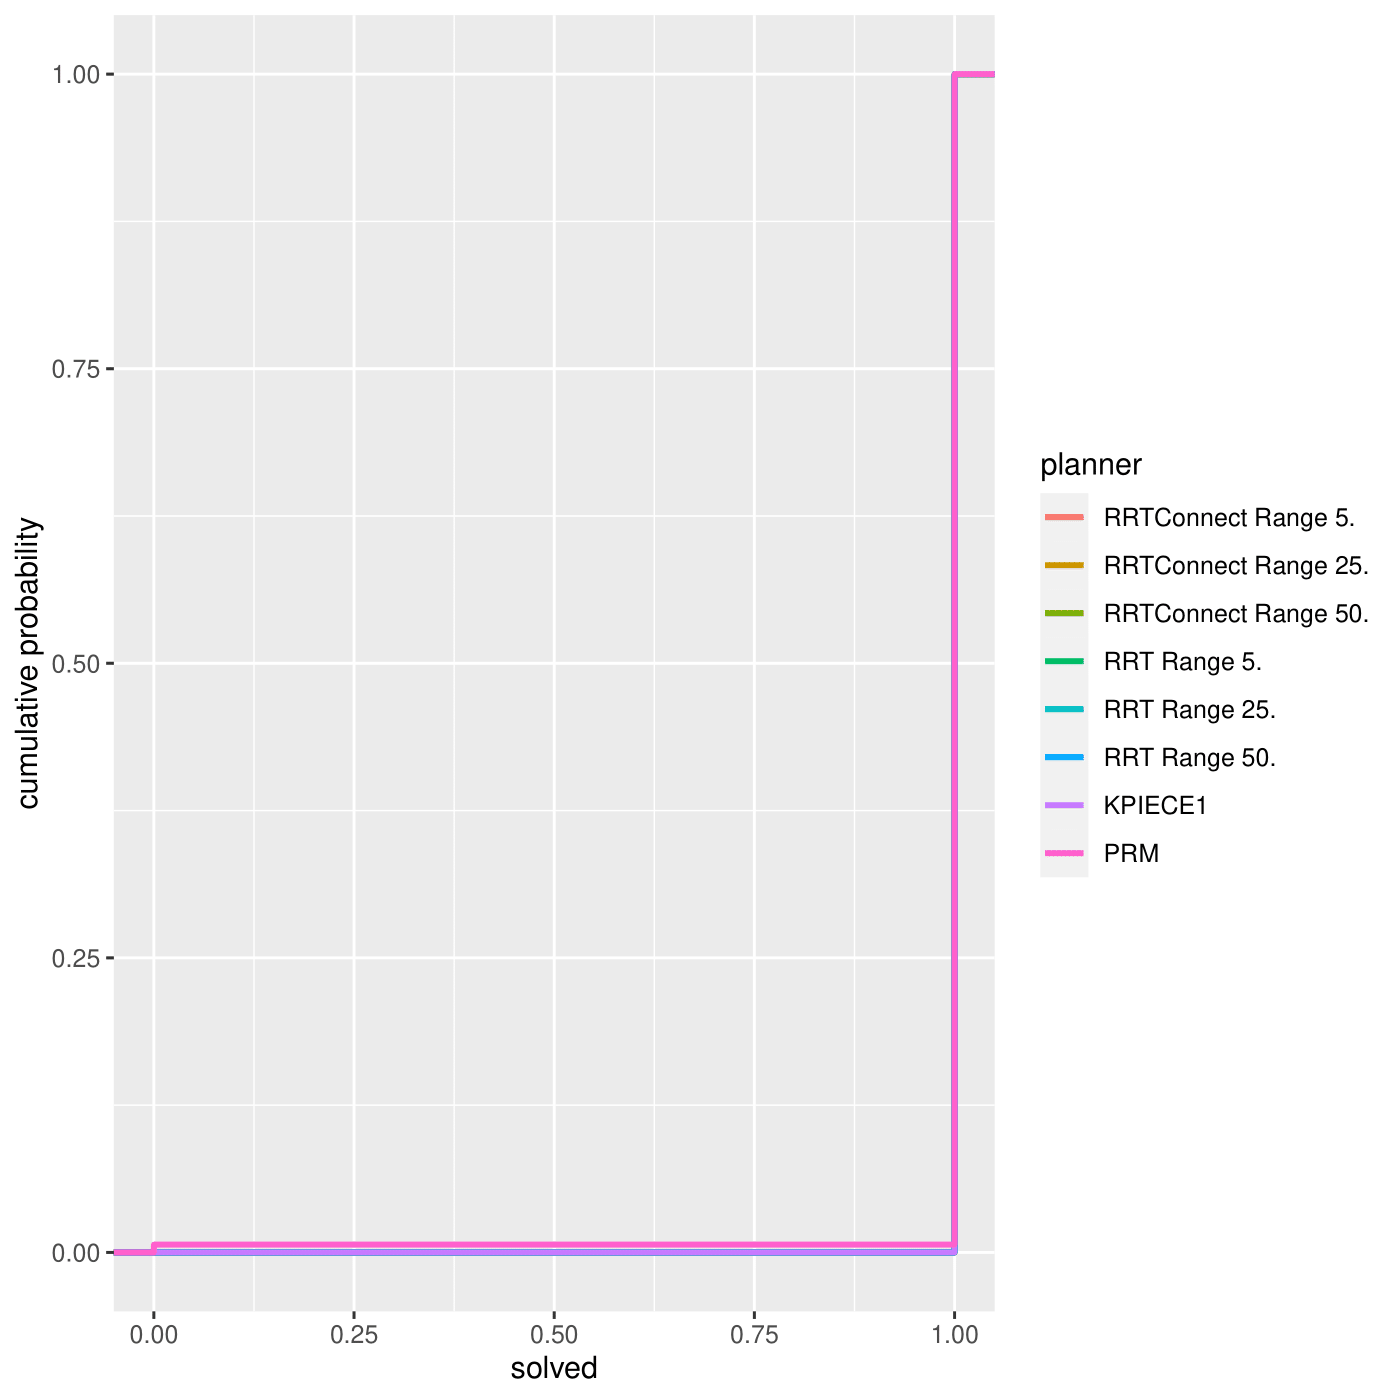
\includegraphics[width=\textwidth]{figures/twistycool_solved-1.png}
              \caption{TwistyCool}
           \end{subfigure}
           \begin{subfigure}[b]{0.3\textwidth}
              \centering
              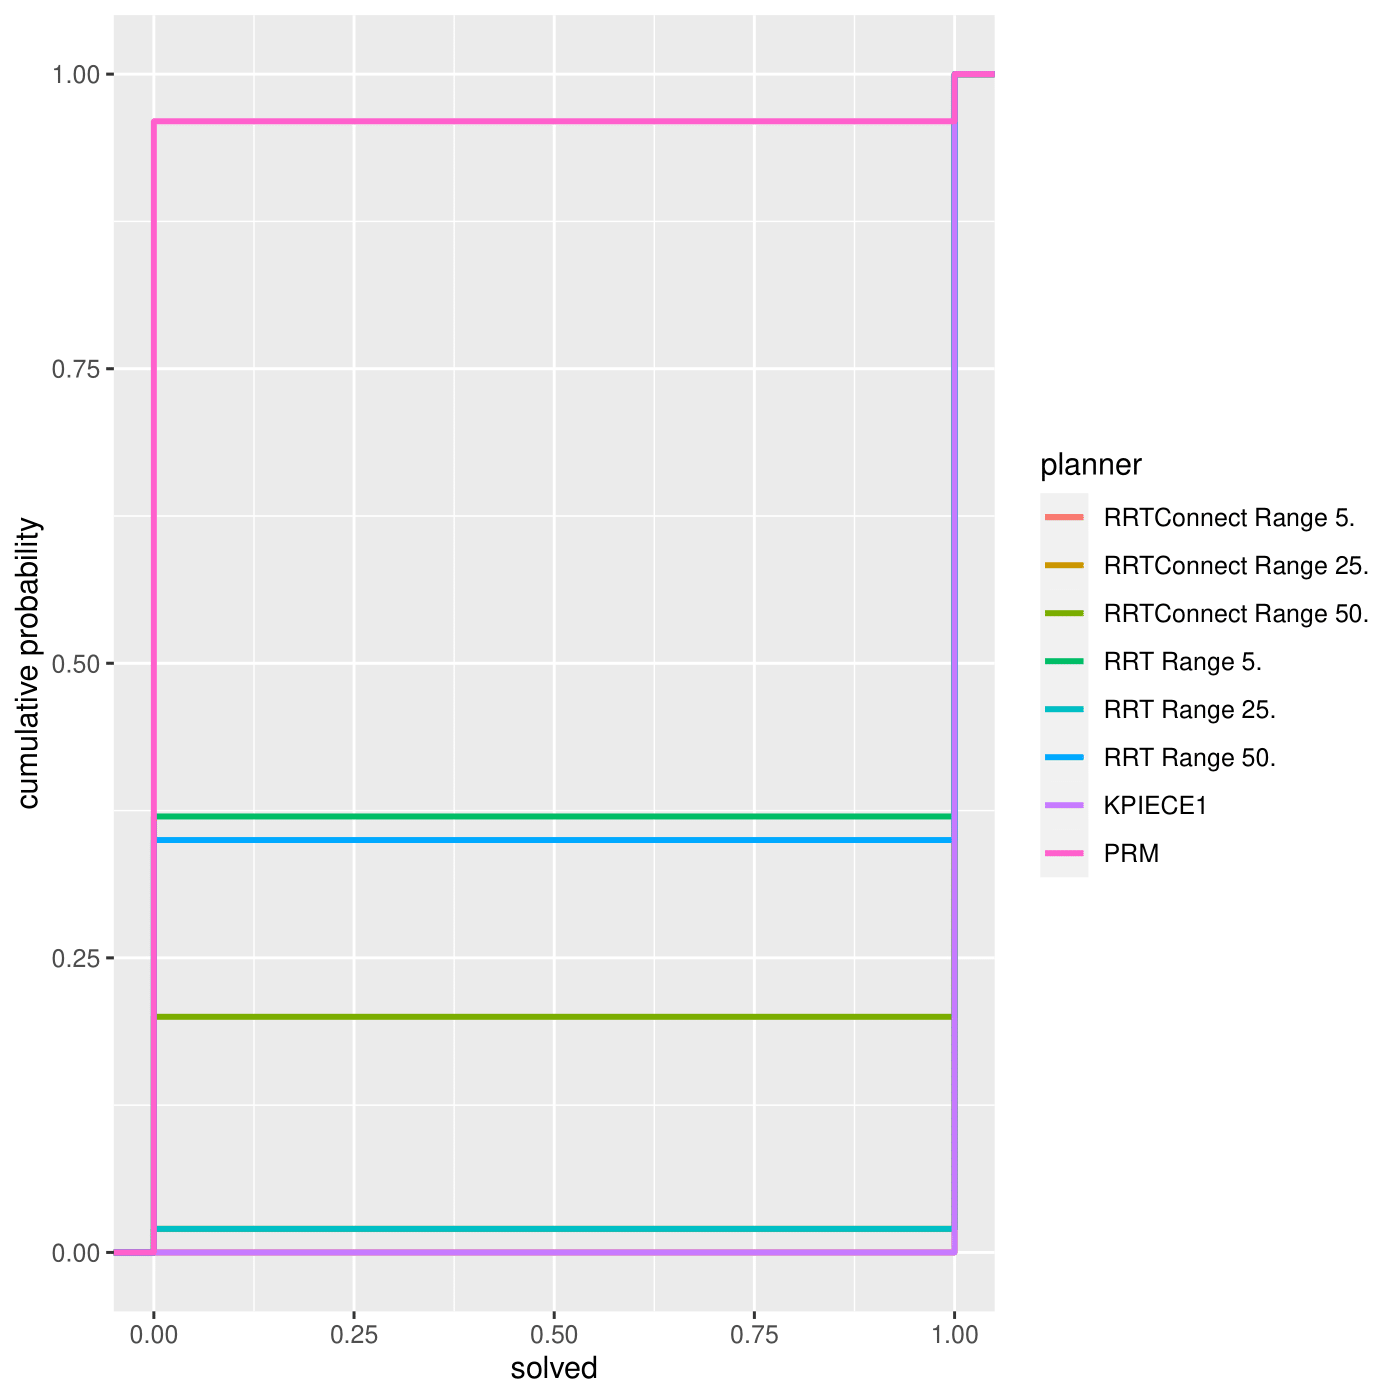
\includegraphics[width=\textwidth]{figures/abstract_solved-1.png}
              \caption{Abstract}
           \end{subfigure}
       \caption{Solved Statistics for Each Problem Configuration}
       \label{fig:1}
       \end{figure}

  \forceindent Since the \text{\fontfamily{cmtt}\selectfont TwistyCool} problem configuration had the best data, with all planners having a success rate of 90 \% or higher to obtain an exact solution for each planner, we can compare the planners for this problem.

  \forceindent First, we can examine the solution length for each planner. These results are summarized below in Figure \ref{fig:2}. For the planners except \text{\fontfamily{cmtt}\selectfont KPIECE1}, similar performance for the solution path length is obtained. The \text{\fontfamily{cmtt}\selectfont RRT} planner with a range of 5 was able to obtain the shortest solution path. \text{\fontfamily{cmtt}\selectfont KPIECE1} planner had the longest average path length, but had a much smaller distribution compared to the other planners. Since \text{\fontfamily{cmtt}\selectfont KPIECE1} does not do statistical sampling like the other 3 planners, a smaller distribution of solution paths is expected.

  \begin{figure}[H]
        \centering
        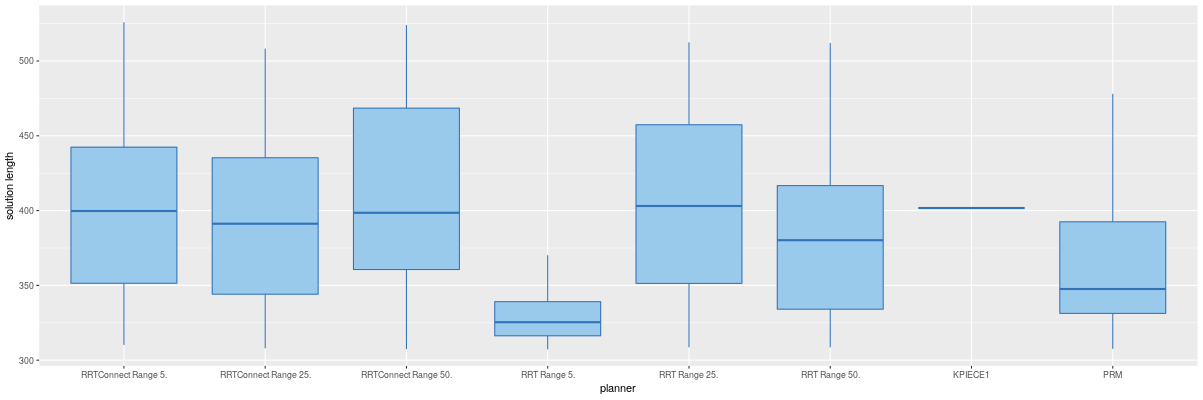
\includegraphics[width=12cm]{figures/twistycool_solnlength-1.png}
        \caption{TwistyCool Solution Length}
        \label{fig:2}
    \end{figure}

\forceindent Next, the time to compute a solution for each planner can be compared. The benchmark results are summarized below in Figure \ref{fig:3}. From examining Figure \ref{fig:3}, the \text{\fontfamily{cmtt}\selectfont RRT} and \text{\fontfamily{cmtt}\selectfont RRT-Connect} planners at ranges 5 and 15 used the lowest time to compute a solution on average. The \text{\fontfamily{cmtt}\selectfont KPIECE1} planner had the highest upper quartile and average time to compute a solution. Additionally, the \text{\fontfamily{cmtt}\selectfont PRM} planner had performance slightly better than \text{\fontfamily{cmtt}\selectfont KPIECE1}. 
    
    \begin{figure}[H]
        \centering
        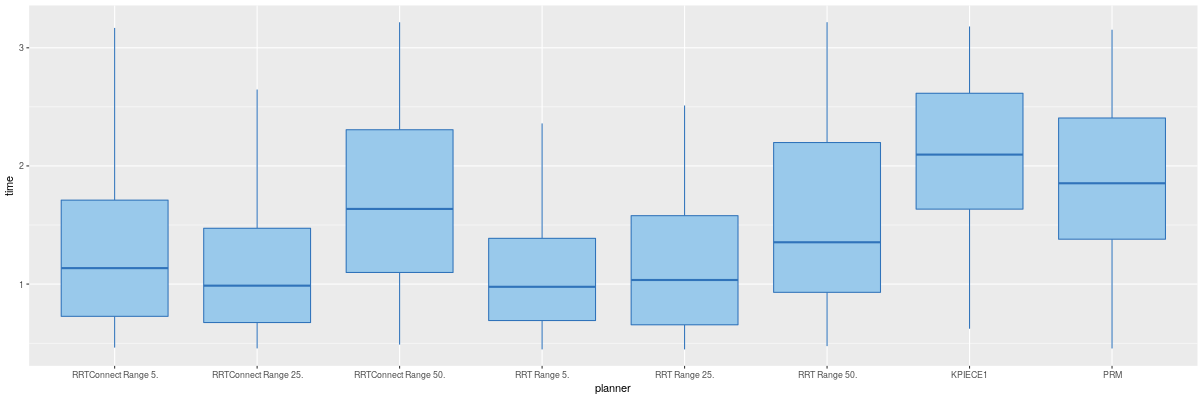
\includegraphics[width=12cm]{figures/twistycool_time-1.png}
        \caption{TwistyCool Time to Compute Solution}
        \label{fig:3}
    \end{figure}

\forceindent Lastly, the number of graph states is compared for the TwistyCool problem. The benchmark results are given in Figure \ref{fig:4}. The \text{\fontfamily{cmtt}\selectfont RRT} and \text{\fontfamily{cmtt}\selectfont RRT-Connect} planners at a range of $10$ and \text{\fontfamily{cmtt}\selectfont PRM} had the best performance with the fewest average graph states, while \text{\fontfamily{cmtt}\selectfont KPIECE1} had the worst performance with most average graph states.     
    
    \begin{figure}[H]
        \centering
        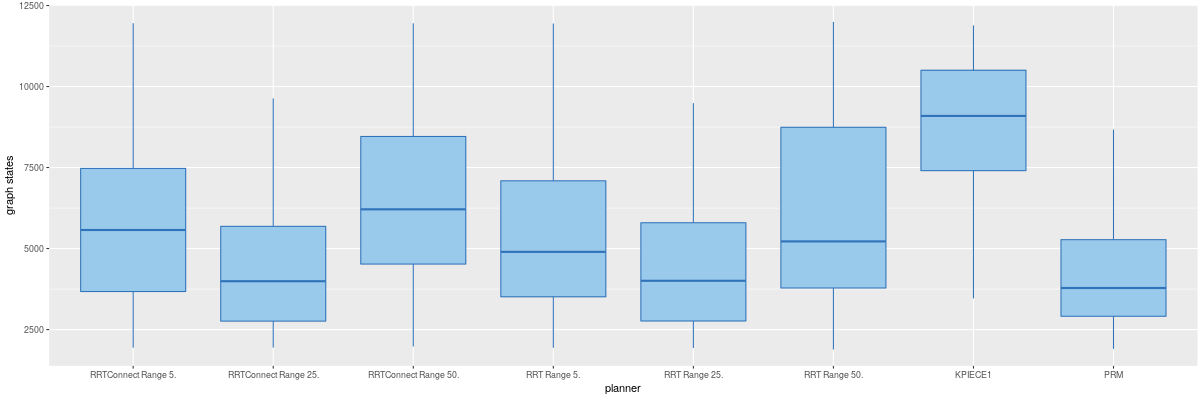
\includegraphics[width=12cm]{figures/twistycool_graphstates-1.png}
        \caption{TwistyCool Number of Graph States}
        \label{fig:4}
    \end{figure}
 
    \forceindent Overall, for the TwistyCool problem configuration, the \text{\fontfamily{cmtt}\selectfont KPIECE1} planner had the worst performance across the three metrics discussed here: solution path length, time to compute solution, and number of graph states. This result is likely because \text{\fontfamily{cmtt}\selectfont KPIECE1} offers a tree-based planner with reliable performance, but it cannot take advantage of variations in how the free workspace is sampled to achieve high performance in some scenarios.
\forceindent The \text{\fontfamily{cmtt}\selectfont RRT} and \text{\fontfamily{cmtt}\selectfont RRT-Connect} planners at a range of $10$ had consistently good performance across the three metrics. Both the average and lower quartile performance outpaced the other planner for time to compute solution and number of graph states. This performance result with a range value of $10$ suggest there is an optimal range value that needs to be tuned when using these planners for a problem. 

   \end{enumerate}    
   
   \item % Problem 7
   \begin{enumerate}[leftmargin=0.3in]
    Problems 1,2,3,4, and 5 had a difficulty of 2. Running the OMPL demos and problems with the GUI was straightforward. Problem 6 had a difficulty of around 8. This difficulty is attributed to the fact that I could not get good benchmark results for complicated problems due to limitation of my hardware, not matter how long I made the runtime.
   \end{enumerate}    

\end{enumerate}

\end{document}
